\documentclass[tikz,border=2pt]{standalone}
\usepackage{amsmath,amssymb}
\usetikzlibrary{arrows.meta}
\begin{document}
% Five jobs: A = (0,1,2.5,6,7.5), D = (2,4,5,7,9). Between A(t) (blue) and D(t) (red),
% job k occupies the strip [A_k, D_k) x [k-1, k] of length J_k = 2, 3, 2.5, 1, 1.5.
% Area = sum J_k = 10 = integral of L over [0,9]; lambda = 5/9, mean J = 2, mean L = 10/9.
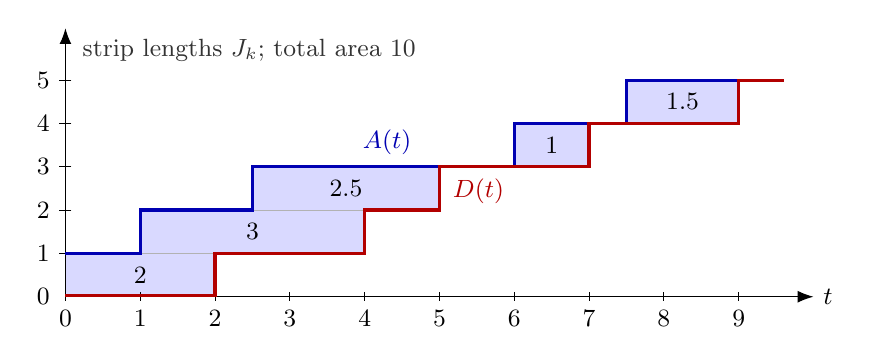
\begin{tikzpicture}[font=\small, >={Latex[length=2mm]}, x=0.95cm, y=0.55cm]
  % strips
  \foreach \a/\d/\k/\j in {0/2/1/2, 1/4/2/3, 2.5/5/3/2.5, 6/7/4/1, 7.5/9/5/1.5}
    {\fill[blue!15] (\a,\k-1) rectangle (\d,\k);
     \draw[gray!60, thin] (\a,\k-1) rectangle (\d,\k);
     \node at ({(\a+\d)/2},\k-0.5) {$\j$};}
  % axes
  \draw[->] (0,0) -- (10,0) node[right] {$t$};
  \draw[->] (0,0) -- (0,6.2);
  \foreach \y in {1,...,5} {\draw (0.08,\y) -- (-0.08,\y) node[left] {$\y$};}
  \node[left] at (-0.08,0) {$0$};
  \foreach \x in {0,1,2,...,9} {\draw (\x,0.1) -- (\x,-0.1) node[below] {$\x$};}
  % arrival process
  \draw[blue!70!black, very thick] (0,1) -- (1,1) -- (1,2) -- (2.5,2) -- (2.5,3) -- (6,3)
    -- (6,4) -- (7.5,4) -- (7.5,5) -- (9.6,5);
  \node[blue!70!black, anchor=south] at (4.3,3.05) {$A(t)$};
  % departure process
  \draw[red!70!black, very thick] (0,0.03) -- (2,0.03) -- (2,1) -- (4,1) -- (4,2) -- (5,2) -- (5,3)
    -- (7,3) -- (7,4) -- (9,4) -- (9,5) -- (9.6,5);
  \node[red!70!black, anchor=north west] at (5.05,2.95) {$D(t)$};
  \node[gray!40!black, anchor=west] at (0.1,5.7) {strip lengths $J_k$; total area $10$};
\end{tikzpicture}
\end{document}
